%%%%%%%%%%%%%%%%%%%%%%%%%%%%%%%%%%%%%%%%%%%%%%%%%%%%%%%%%%%%%%
%															 %
%	IDS main document for bachelor and master thesis		 %
%	created by Jan Richter-Brockmann 						 %
%	Sommersemester 2017										 %
%															 %
%%%%%%%%%%%%%%%%%%%%%%%%%%%%%%%%%%%%%%%%%%%%%%%%%%%%%%%%%%%%%%

\documentclass[
	a4paper,
	12pt,
	twoside=true,
	BCOR10mm,					% Bindekorrektur
	toc=bibliography,			% Fuegt das Literaturverzeichnis ins Inhaltsverzeichnis ein
	cleardoublepage=empty
]{scrbook}

\usepackage[utf8]{inputenc}


%%%%%%%%%%%%%%%%%%%%%%%%%%%%%%%%%%%%%%%%%%%%%%%%%%%%%%%%%%%%%%
%															 %
%	Conditionals											 %
%															 %
%%%%%%%%%%%%%%%%%%%%%%%%%%%%%%%%%%%%%%%%%%%%%%%%%%%%%%%%%%%%%%

\usepackage{ifthen}
\newboolean{Confidential}
\newboolean{EnglishVersion}
\newboolean{Logo}
\newboolean{PrintedVersion}

% Edit this file to set your personal information
%%%%%%%%%%%%%%%%%%%%%%%%%%%%%%%%%%%%%%%%%%%%%%%%%%%%%%%%%%%%%%
%															 %
%	Settings												 %
%	Change the settings of your work here				 	 %
%															 %
%%%%%%%%%%%%%%%%%%%%%%%%%%%%%%%%%%%%%%%%%%%%%%%%%%%%%%%%%%%%%%

\setboolean{EnglishVersion}{false}
\setboolean{PrintedVersion}{false}

\newcommand{\IDSAuthorFirstName}{Arthur}
\newcommand{\IDSAuthorSecondName}{Ruder}
\newcommand{\IDSTitleGerman}{Industriepraktikum bei Enclustra FPGA Solutions, Räffelstrasse 28, CH-8045 Zürich}
\newcommand{\IDSTitleEnglish}{Industriepraktikum bei Enclustra FPGA Solutions, Räffelstrasse 28, CH-8045 Zürich}
\newcommand{\IDSSubject}{Praktikumsbericht}% Bachelorarbeit, Studienarbeit usw.
\newcommand{\IDSMatNr}{310697}
\newcommand{\IDSSupervisor}{Martin Heimlicher}
\newcommand{\IDSNumber}{}
\newcommand{\IDSSubmissionDate}{06.09.2019}

% Changes First Page to use No Logo
% \setboolean{NoLogo}{true}

% Please look at http://www.rwth-aachen.de/go/id/hjxv
% or search for "Hinweise zu schriftlichen Arbeiten an der RWTH" 
% to get the "Erklärung zur Verwendung des logos" and reache it in to "ZPA"


%\graphicspath{{bilder/}} %relativer Pfad, in dem die Bilder liegen


%\bibliography{Ref}IDSAuthorSecondName

\ifthenelse{\boolean{EnglishVersion}}{
	\usepackage[english]{babel}
}{
	\usepackage[ngerman]{babel}
}


%%%%%%%%%%%%%%%%%%%%%%%%%%%%%%%%%%%%%%%%%%%%%%%%%%%%%%%%%%%%%%
%															 %
%	Page layout												 %
%															 %
%%%%%%%%%%%%%%%%%%%%%%%%%%%%%%%%%%%%%%%%%%%%%%%%%%%%%%%%%%%%%%

\usepackage[headsepline]{scrpage2}
\pagestyle{scrheadings}
\setheadsepline{0.5pt}

\usepackage[onehalfspacing]{setspace}
\usepackage{microtype}	% Nicer spacings, prevents to cross the page's margin


%%%%%%%%%%%%%%%%%%%%%%%%%%%%%%%%%%%%%%%%%%%%%%%%%%%%%%%%%%%%%%
%															 %
%	Images, formulas and tables								 %
%															 %
%%%%%%%%%%%%%%%%%%%%%%%%%%%%%%%%%%%%%%%%%%%%%%%%%%%%%%%%%%%%%%

\usepackage{subfigure}	
\usepackage{pgfplots}
\usepackage{graphicx}
\usepackage{tikz}	% this package become very handy when plotting graphs 
\usepackage{tikz-timing}
\usepackage{circuitikz}
\usetikzlibrary{external}
\usetikzlibrary{patterns}
\usetikzlibrary{shapes.geometric}
\tikzexternalize[prefix=tikzplot/]
\usepackage{xintexpr}

\usepackage[tbtags]{amsmath}
\usepackage{amsfonts}
\usepackage{trfsigns}	% Laplace symbol 
\usepackage{gensymb}

\usepackage{array}
\usepackage{booktabs}
\usepackage{multirow}
\usepackage{tabularx}
\usepackage{longtable}

% Colors - use plot1 - plot7 for your plots
% IDSblua can be used for figures
\definecolor{IDSblue}{rgb}{0,0.3294118,0.623529}%
\definecolor{plot1}{rgb}{0,0.3294118,0.623529}%
\definecolor{plot2}{rgb}{1,0,0}%
\definecolor{plot3}{rgb}{0.647058824,0.647058824,0.647058824}%
\definecolor{plot4}{rgb}{0.498,0.788,0.498}%
\definecolor{plot5}{rgb}{0.745,0.682,0.831}%
\definecolor{plot6}{rgb}{0.941,0.007,0.498}%
\definecolor{plot7}{rgb}{0.749,0.357,0.09}%


%%%%%%%%%%%%%%%%%%%%%%%%%%%%%%%%%%%%%%%%%%%%%%%%%%%%%%%%%%%%%%
%															 %
%	Unities													 %
%															 %
%%%%%%%%%%%%%%%%%%%%%%%%%%%%%%%%%%%%%%%%%%%%%%%%%%%%%%%%%%%%%%

\usepackage[load-configurations=binary, load-configurations=abbreviations]{siunitx}
\ifthenelse{\boolean{EnglishVersion}}{
	\sisetup{group-separator = {,}}
}{
	\sisetup{group-separator = {.}}
}
\sisetup{group-minimum-digits = 3}


%%%%%%%%%%%%%%%%%%%%%%%%%%%%%%%%%%%%%%%%%%%%%%%%%%%%%%%%%%%%%%
%															 %
%	References												 %
%															 %
%%%%%%%%%%%%%%%%%%%%%%%%%%%%%%%%%%%%%%%%%%%%%%%%%%%%%%%%%%%%%%

\usepackage[style=numeric-verb, backend=bibtex8]{biblatex}
\addbibresource{Ref.bib}


%%%%%%%%%%%%%%%%%%%%%%%%%%%%%%%%%%%%%%%%%%%%%%%%%%%%%%%%%%%%%%
%															 %
%	Misc													 %
%															 %
%%%%%%%%%%%%%%%%%%%%%%%%%%%%%%%%%%%%%%%%%%%%%%%%%%%%%%%%%%%%%%

\usepackage[hidelinks]{hyperref}	% Enables links in the PDF
\usepackage[printonlyused]{acronym}
\renewcommand*{\acffont}[1]{{\color{black}\itshape{#1}}}
\usepackage{pdfpages}
\usepackage{algorithm}				% see algorithm documentation to use this package
\usepackage[]{algpseudocode}
\usepackage{pdflscape}




%%%%%%%%%%%%%%%%%%%%%%%%%%%%%%%%%%%%%%%%%%%%%%%%%%%%%%%%%%%%%%
%															 %
%	Main-Document											 %
%															 %
%%%%%%%%%%%%%%%%%%%%%%%%%%%%%%%%%%%%%%%%%%%%%%%%%%%%%%%%%%%%%%

\begin{document}
	%%%%%%%%%%%%%%%%%%%%%%%%%%%%%%%%%%%%%%%%%%%%%%%%%%%%%%%%%%%%%%
%															 %
%	Titel Page												 %
%															 %
%%%%%%%%%%%%%%%%%%%%%%%%%%%%%%%%%%%%%%%%%%%%%%%%%%%%%%%%%%%%%%

\begin{titlepage}

\pagestyle{empty}

\ifthenelse{\boolean{EnglishVersion}}{
	\pdfbookmark[0]{Front Page}{Front Page}
}{
	\pdfbookmark[0]{Titelseite}{Titelseite}
}

\enlargethispage{2.3in}
\setlength{\voffset}{-1in}

\hspace*{3cm}
\begin{flushright}

\includegraphics[height=25mm]{bilder/ids_logo/rwth_ids_en_rgb.png}
\end{flushright}
%\bigskip
\setcounter{subfigure}{0}

%~\\
%\ifthenelse{\boolean{EnglishVersion}}{
%	The present work was submitted to the Chair of Integrated Digital Systems and Circuit Design.
%}{
%	Diese Arbeit wurde vorgelegt am Lehrstuhl für Integrierte Digitale Systeme und Schaltungen der RWTH Aachen.
%}
 
\vspace{15mm}

{ \centering \huge \MakeUppercase \IDSSubject \\} 

\vspace{15mm}

{\color{IDSblue}\hrule}\par
\vspace{1mm}
{\color{IDSblue}\hrule}\par

\bigskip 

~\\
\ifthenelse{\boolean{EnglishVersion}}{
	{\LARGE \bfseries \centering \IDSTitleEnglish \\}	
}{
	{\LARGE \bfseries \centering \IDSTitleGerman \\}		
}
~\\

{\color{IDSblue}\hrule}\par
\vspace{1mm}
{\color{IDSblue}\hrule}\par


%{\usefont{\encodingdefault}{cpc}{m}{n}\selectfont \Large \MakeUppercase \IDSSubject \\} \bigskip
\vspace{5mm}
~\\
\begin{raggedleft}
\ifthenelse{\boolean{EnglishVersion}}{
	{\Large presented by\\}
}{
	{\Large von\\}
}
~ {\Large   \IDSAuthorFirstName~\IDSAuthorSecondName\\}
{\Large Matr.-Nr. \IDSMatNr \\} 

\par \vspace*{\fill}

\bigskip \bigskip

%~\\~\\~\\
%\ifthenelse{\boolean{EnglishVersion}}{
%	{\large  Supervised by \IDSSupervisor \\}
%	~\\
%	{\large reviewed by Prof.\ Dr.-Ing.\ Tobias Gemmeke \\}
%}{
%	{\Large Unter der Betreuung von \IDSSupervisor \\}
%}


\bigskip \bigskip

%~\\
%\ifthenelse{\boolean{EnglishVersion}}{
	%{\Large $1^{st}$ Examiner: Prof. Dr.-Ing. Tobias Gemmeke}
%	~\\
	%{\Large $2^{nd}$ Examiner: ---}
%}{
%	{\Large 1. Prüfer: Prof. Dr.-Ing. Tobias Gemmeke}
%	~\\
%	{\Large 2. Prüfer: ---}
%}
\end{raggedleft}
\bigskip
~\\

{\flushright{ \Large Aachen, \IDSSubmissionDate}\\~\\}


\newpage
\setlength{\voffset}{0in}


\thispagestyle{empty}
\rule{0pt}{0pt}
\cleardoublepage

\end{titlepage}
	\cleardoubleemptypage
	
	% ------------------------------------------------------------------------------------
	% Table Of Contents
	\tableofcontents
	\cleardoubleemptypage
	\phantomsection			% is required to neglect this chapter in the TOC
	
	% ------------------------------------------------------------------------------------
	% List of Figures
	\addcontentsline{toc}{chapter}{List of Figures}
	\listoffigures
	\cleardoubleemptypage
	
	% ------------------------------------------------------------------------------------
	% List of Tables
	\addcontentsline{toc}{chapter}{List of Tables}
	\listoftables
	\cleardoubleemptypage
	
	% ------------------------------------------------------------------------------------
	
	\pagenumbering{arabic}	% change the numbering to arabic numbers
	
	% CONTENT - include all your content files in content.tex
	% Add your content here

%%%%%%%%%%%%%%%%%%%%%%%%%%%%%%%%%%%%%%%%%%%%%%%%%%%%%%%%%%%%%%
%																
%	Chapter 1 - Introduction and Motivation 															 
%																				 
%%%%%%%%%%%%%%%%%%%%%%%%%%%%%%%%%%%%%%%%%%%%%%%%%%%%%%%%%%%%%%

\chapter{Week 1}
\chapter{Week}
At the beginning of the week a task unrelated to \ac{AI} was given to check upon internal documentation and customer support. Together with another recently hired employee, a day of out-of-box testing was scheduled. An Enclustra base board (Mercury+ PE1-400) together with a fitting \ac{FPGA} module (Mercury+ XU1) featuring a Xilinx \ac{MPSoC}.
Some details will be given for this specific \ac{FPGA} family as the Zynq-7000 \ac{SoC} and the Zynq-\ac{MPSoC} Xilinx product family are unique in the way dedicated ARM processors are combined with traditional \acp{FPGA}. A high level overview is shown in figure~\ref{fig:zynq-overview}.
\begin{figure}[!htb]
	\centering
		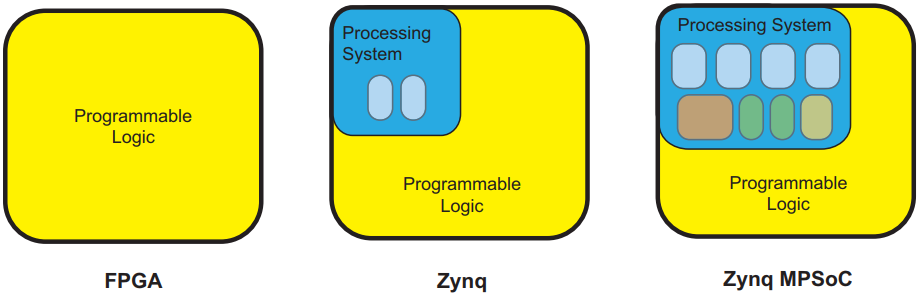
\includegraphics[width=\textwidth]{bilder/ZYNQ-overview.png}
		\caption{High level ZYNQ family overview~\cite{zynq-book}}
		\label{fig:zynq-overview}
\end{figure}
It shows the difference between traditional \acp{FPGA} and the Zynq product family. The main benefit here is the division between \ac{PS} and \ac{PL}. This allows to combine the benefits of traditional processing units with the flexibility of \acp{FPGA}. Custom logic and all peripheral devices can be implemented in the \ac{PL} part, while system control and even complete \acp{OS} (such as embedded Linux) can be done in the \ac{PS}. As this system is completely integrated in one package, the communication between the two fabrics is extremely fast and can be done using \ac{AXI} interfaces. The \ac{MPSoC} family even integrates several different types of processing units, \acp{APU}, \acp{GPU}, \acp{VPU} and \acp{RPU}.
The Enclustra module uses an \ac{MPSoC} Xilinx FPGA and our task was to go through the whole process of bringing up the base board together with a corresponding module to test customer experience using the provided documentation, user manual and reference design. The goal was to find unclear instructions in the documentation and provide feedback as to the overall experience bringing up the hardware out-of-the-box. First, the hardware reference design was loaded in the Vivado Design Suite and the bit stream generated. After, the hardware description file was exported so it can be used using the Xilinx \ac{SDK}. This allows to create applications in C/C++ against the custom hardware design. All of the provided sample applications have been tested and verified. Some unclear instructions were identified and discussed with the employee in charge to improve customer experience.
The rest of the week was spend updating the internal Wiki page for \ac{AI}. Furthermore, the \ac{DNNDK} sample applications were tested on the ZCU 104 evaluation board. The provided examples include several state-of-the-art neural networks demonstrating key applications for neural network inference, such as image classification, face detection, object detection and pose detection. As only the image classification example worked directly for this particular evaluation a fix needed to be found. Another task was to introduce the topic of \ac{AI} to the whole company as \acp{ANN} was a completely new design field for a majority of the technical staff. Two PowerPoint presentations should be prepared, namely 'Introduction to \ac{AI}' and 'Introduction to \ac{ML} on \acp{FPGA}'. I started with the preparation of the first one in parallel with finding a bug fix for the other \ac{DNNDK} sample applications, as these should be part of the second presentation.
\chapter{Week}
The main focus of this week was research and starting to layout the first presentation. It was assumed that the audience is technology savvy but has no particular background in \ac{AI}. Thus, the presentation had to introduce the whole field and key concepts that enabled the rise of \ac{AI} applications in recent years. The first draft of the presentation was discussed in a meeting and some changes were made to the overall structure, the content and the degree of complexity.The rough structure of the presentation is as follows:
\begin{itemize}
	\item \textbf{Motivation}: To get the viewers interest it was shown that \ac{AI} applications are already part of daily life for everyone. This was achieved by showing that all of the major companies such as Google, Apple, Facebook, Microsoft as well as Tesla, Netflix and Amazon use \ac{AI} in their datacenters and products and allocate huge resources to \ac{AI} research. The importance of \ac{AI} was further enhanced by showing the rapid growth of annually published \ac{AI} papers and startups developing \ac{AI} systems. The trend from 1995 to 2015 resembles almost exponential growth in \ac{AI} research and products.
	\item \textbf{Definition}: As \ac{AI} has become such a buzz word in media a definition of the term was needed and what part of \ac{AI} is actually used in all of the common applications. \ac{ANN} that perform typical computer vision and language processing tasks are all part of \ac{ML}, which is a subset of \ac{AI}. \ac{ML} itself can then be divided into further subsets using roughly three learning methods, supervised learning, unsupervised learning and reinforcement learning. As supervised learning is the most commonly used method, the presentation focused on this method used to train \ac{ANN}. Furthermore, the different parts that comprise a \ac{ANN} are introduced, namely the neuron and how neurons are formed into layers. These layers are then stacked together to form an \ac{ANN}.
	\item \textbf{Key concepts}: An explanation of supervised learning was given with two distinct examples, linear regression and deep learning neural networks to illustrate the idea behind supervised learning: predict a value $y$ given an input $x$ by deploying a function $f(x)$. This function $f(x)$ is acquired by deploying a learning algorithm and usage of a so called training set, consisting of input pairs $x$ and $y$. The concept of inference and training were also explained with an emphasis on inference. Once a network is trained, only inference needs to be run, so this is the crucial part application wise.
	\begin{figure}[!htb]
	\centering
		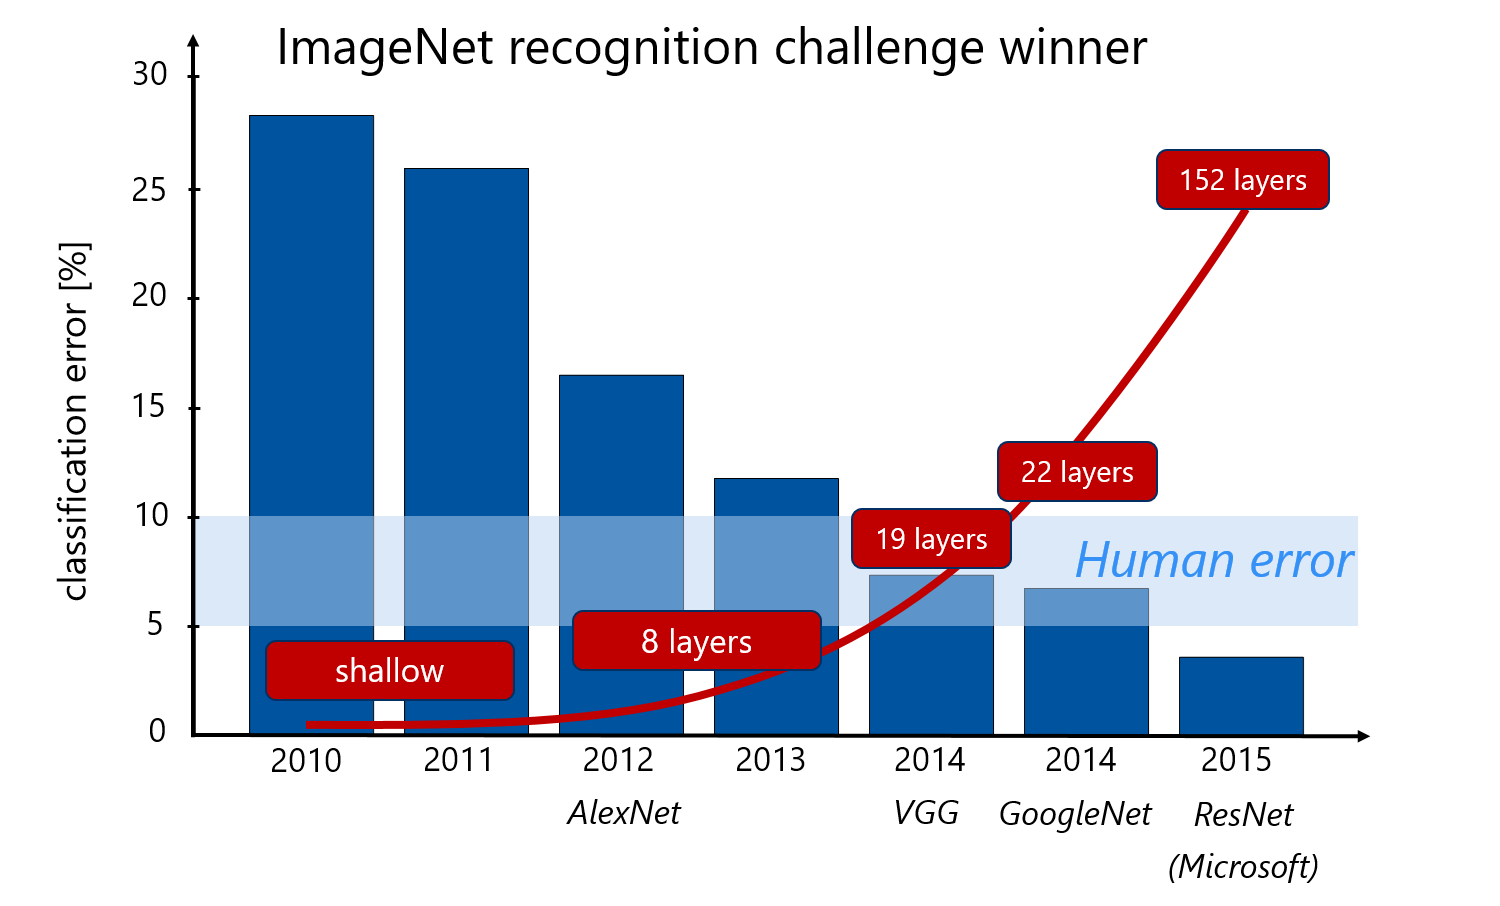
\includegraphics[width=\textwidth]{bilder/ilsvrc.png}
		\caption{ILSVRC winners}
		\label{fig:ilsvrc}
\end{figure}
	\item \textbf{Deep Learning}: Figure~\ref{fig:ilsvrc} shows the winners of the state-of-the-art ImageNet Large Scale Visual Recognition Challenge. It illustrates that the breakthrough in performance came not only from more sophisticated networks, but mainly from stacking different kinds of layers deeply, hence the name. The presentation was ended with the question, what hardware is best suited for \ac{ANN} applications.
\end{itemize}
Alongside preparing the presentation the error preventing the more sophisticated examples was identified as the board crashed while performing tasks related to video analysis (face detection, pose detection, etc.). At first, it was suspected there were some problems with heat management and using the system monitor the temperature of the \ac{FPGA} was investigated during operation. As this seemed to be well within allowed borders specified by the Xilinx data sheet, other causes had to be found.
\chapter{Week}
At the beginning of the week the first presentation 'Introduction to \ac{AI}' was held before the technical stuff of the company. The general background and principles of \ac{ML} have been introduced and an outlook given to the second presentation, which would go more into detail about the actual hardware realization. The rest of the week was spent going through various tutorials provided by Xilinx to familiarize myself with the workflow and the \ac{DNNDK} toolkit. As the state of tools used for \ac{AI} applications on \ac{FPGA} is still in flux, several approaches needed to be evaluated:
\begin{itemize}
	\item \textbf{\ac{DNNDK} workflow}: Version 2.08 of the toolkit supported only the Caffe neural network training framework and needs a network description file and the trained weights as input. The key component here is the \ac{DPU} \ac{IP} core provided by the \ac{DNNDK} toolkit. This core is integrated via Vivado into the block design of the hardware and can be configured and adjusted for several performance and power profiles.
	\item \textbf{\ac{DNNDK} \ac{SDSoC}}: Another option is to abstract away the whole Vivado block design process and use Xilinx \ac{SDSoC} to implement the whole system in a higher programming language, C++. Supported functions can then be flagged as being executed in the \ac{PL} part of the system. This approach makes using a traditional \ac{HDL} obsolete and is deemed more accessible. This approach uses the established Xilinx reVision stack for development providing high level \acp{API} for computer vision.
\end{itemize}
Furthermore, the \ac{IP} core provided by the \ac{DNNDK} toolkit was studied in more detail. A new base board was in the production state phase and the idea was to have a \ac{ML} design ready to showcase the capabilities of the new board.
\begin{figure}[!htb]
	\centering
		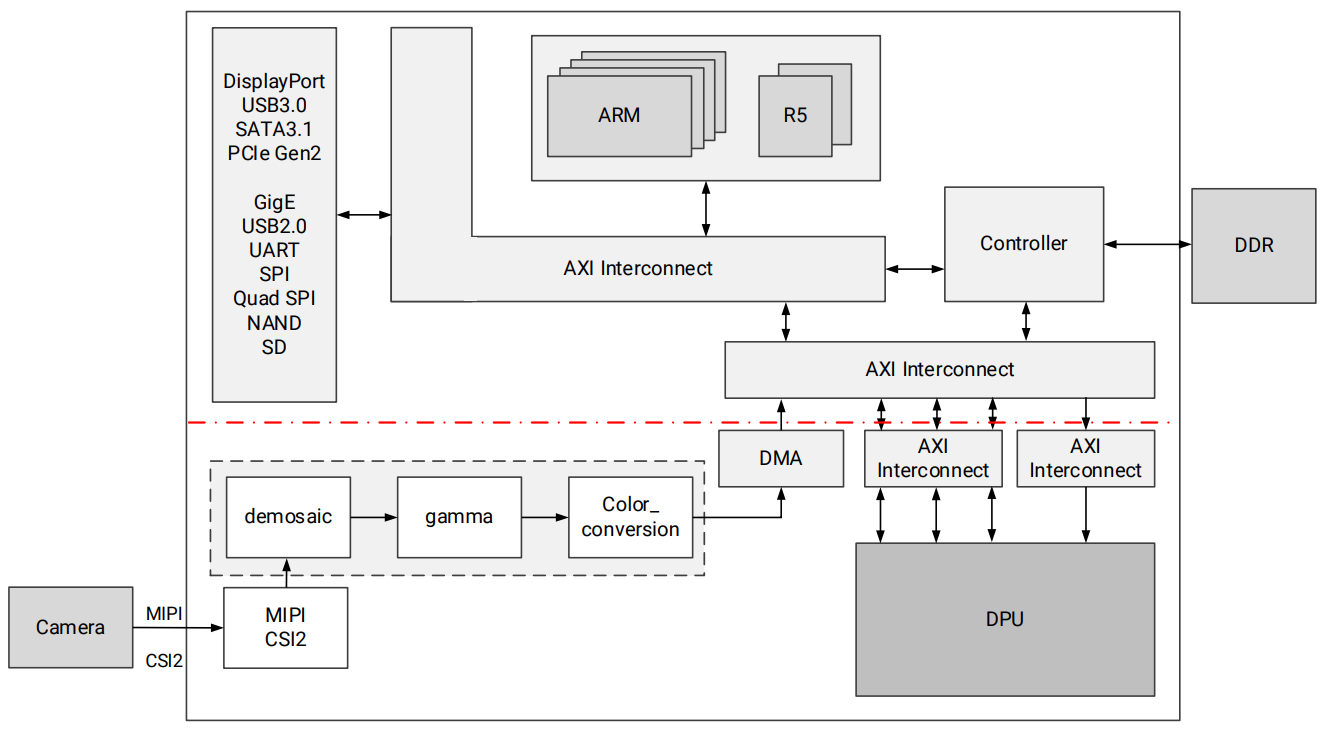
\includegraphics[width=\textwidth]{bilder/DPU_example_design.png}
		\caption{Example system with integrated \acs{DPU} \cite[p.~8]{dpu}}
		\label{fig:dpu_example}
\end{figure}
Figure~\ref{fig:dpu_example} shows an example hardware design with integrated \ac{DPU} module. In this example a camera is connected via the \ac{MIPI} \ac{CSI2} interface to the \ac{PS}. \ac{DMA} is usually used in conjunction with an \ac{AXI} interconnect to communicate with the \ac{PS}. The captured images are used as the input to the neural network and the \ac{DPU} itself can be viewed as a co-processor to the \ac{PS} implemented in the \ac{PL} fabric. The \ac{IP} core itself is customizable and the number of \ac{DPU} processor units, the size of the \ac{DPU} and the usage of \ac{DSP} blocks among other parameters are configurable. The decision on which size to use is based upon the performance demands of the application.
\chapter{Week}
In this week I started working on the second presentation 'Introduction to \ac{ML} on \acp{FPGA}'. This time the focus should be on the hardware needed to handle typical \ac{ML} workloads, namely inference and training along all major fields of applications where \ac{ANN} are used. The main areas are: image classification, object detection, semantic segmentation, optical character recognition and speech recognition. The presentation structure is as follows:
\begin{itemize}
	\item \textbf{\ac{ANN} workload:} Using a state-of-the-art neural network (resnet50) the number of operations per image were illustrated to show the vast amount of compute and memory needed for a single image. This was done for inference and training respectively with the purpose of driving home the challenges involved in \ac{ML} applications. Moreover, the majority of operations are costly \ac{MAC} operations which take several clock cycles to complete.
	\item \textbf{Hardware for training:} The industry right now in terms of \ac{ANN} training is dominated by NVIDIA and so the clear answer here was \ac{GPU}. There are a number of start-ups developing alternative solutions to get into the \ac{ANN} training market. The main advantage these start-ups have is that they can design from scratch and use an architecture tailored to the specific requirements of \ac{ANN} training. The sheer number of floating point 32 operations and the requirements for memory are strictly not suited for \acp{FPGA}.
	\item \textbf{Hardware for inference:} The picture is different for inference. Here, a lot of research has been done in using quantization and pruning of \ac{ANN} models without impeding the performance of these networks. The reason for this is, that neural networks are inherently over-parametrized and this is necessary for the training algorithms to work. Once a trained network is obtained however, the network can be compressed severely (up to 90 \%) without network degradation. A qualitative comparison of the available platforms was made to show the strengths and weaknesses of each platform. The flexibility of \acp{FPGA} make them a suitable platform for \ac{ANN} inference.
	\item \textbf{\ac{FPGA} architecture:} Figure~\ref{fig:fpga_arch} shows the two possible high-level architectures that are typically used in neural network implementations. On the left you have the streaming architecture where basically the structure of the neural network is mirrored by the hardware implementation. The main benefit is the efficiency and customizability as the hardware can be tailored specifically to each network. The other approach is shown on the right. This is a more general approach in that it has a single computation engine which breaks down the operations needed for neural network inference. These operations are controlled by a host and executed on demand. The main benefit here is the flexibility. As the types of layers in a neural network are fixed, efficient implementation of these different types of layers enables the deployment of arbitrary neural networks. The downside is that the implementation is limited by the architecture in terms of tailoring the hardware implementation to the neural network.
	\begin{figure}[!htb]
	\centering
		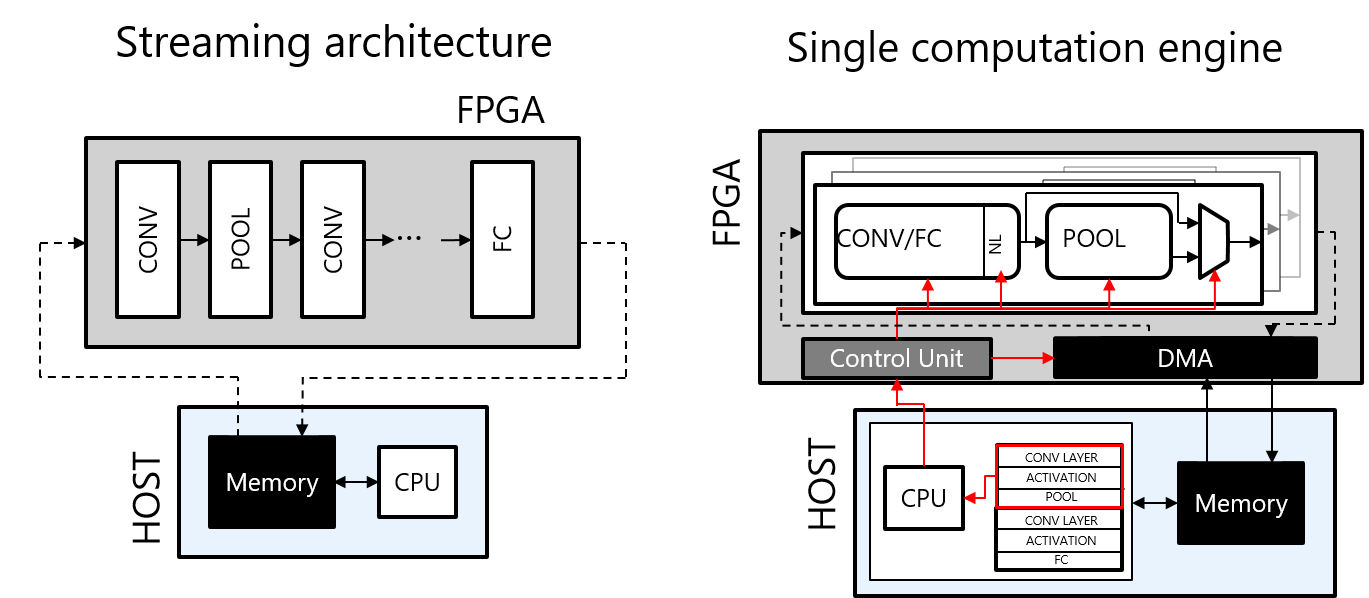
\includegraphics[width=\textwidth]{bilder/FPGA_arch.png}
		\caption{\acs{FPGA} architecture overview}
		\label{fig:fpga_arch}
\end{figure}
	\item \textbf{\ac{DNNDK} work flow:} Lastly, the \ac{DNNDK} work flow is introduced with a focus on adjusting the \ac{DPU} \ac{IP} core to custom boards. Some demonstrations implemented on the ZCU 104 evaluation board were used to finish the presentation and show the employees, what is possible with the tools available.
\end{itemize}
In this week on Thursday there was a Xilinx \ac{ML} seminar in Munich, where I went to with my supervisor to get more information about Xilinx \ac{AI} solutions. This was a whole day event with several segments, showing off the capabilities and the work flow of Xilinx cloud and edge \ac{AI} tools. This was also a great opportunity for networking and speaking in person to top Xilinx \ac{FAE} engineers.
\chapter{Week}
All of the new information gathered at the Xilinx seminar last week needed to be transferred to the internal Wiki and properly documented. Three main tasks were worked upon in this week, namely preparing the second presentation 'Introduction to \ac{ML} on \ac{FPGA}', getting all of the \ac{DNNDK} sample applications to work on the ZCU 104 evaluation board and evaluating a possible collaboration with an ETH start-up called Synthara.
\begin{itemize}
	\item \textbf{Presentation:} Extensive market research has been conducted to find resources and ideas on how to present the different hardware platforms. The difficulty lies therein, that there are no standardized performance metrics for neural networks. Performance is strongly dependent on the network used and the individual use case. This leads to a lot of unfair comparisons, both in research and industry when numbers are shown. Therefore, a qualitative approach was chosen as doing all of these comparisons would have taken an extreme amount of work time and effort, requiring special hardware as well.
	\item \textbf{Bugfix for ZCU 104 evaluation board:} After reading through a vast amount of documentation and employing the help of online resources, mainly the Xilinx official forums, a solution was found to the problem. It turned out to be a specific problem of the ZCU 104 evaluation board which made it hard to track down. The solution to this was provided by an unofficial patch by on e of the Xilinx employees online. The board has power issues when running at full load resulting in the already mentioned problem of freezing the board in the middle of running the sample applications. After applying the patch all of the sample applications worked. These included image classification with resnet50 and inception-v1 as well as real time face detection, object detection and pose detection using other popular \ac{ANN}
	\item \textbf{Synthara collaboration:} During research for neural network accelerator implementations I read about an ETH start-up providing this service in the form of an \ac{ASIC}. However, their prototypes as a proof-of-concept are implemented on \acp{FPGA}. Thus, we reached out to them and scheduled a meeting. During this meeting we discussed the possibility of a cooperation. The idea was to implement a demonstrator for the Embedded World 2020 conference showing off Enclustra hardware and using the Synthara neural network accelerator. The demo is a game of rock-paper-scissors played by a human player against a robotic hand. The setup can be seen in figure~\ref{fig:demonstrator}. The robot hand is controlled via \ac{USB} using \ac{PWM} to control each finger individually. The human players movement is captured by a camera connected via \ac{MIPI} to the \ac{FPGA} board. The \ac{FPGA} handles all image preprocessing and is running a custom neural network capable of detecting hand gestures.
	\begin{figure}[!htb]
	\centering
		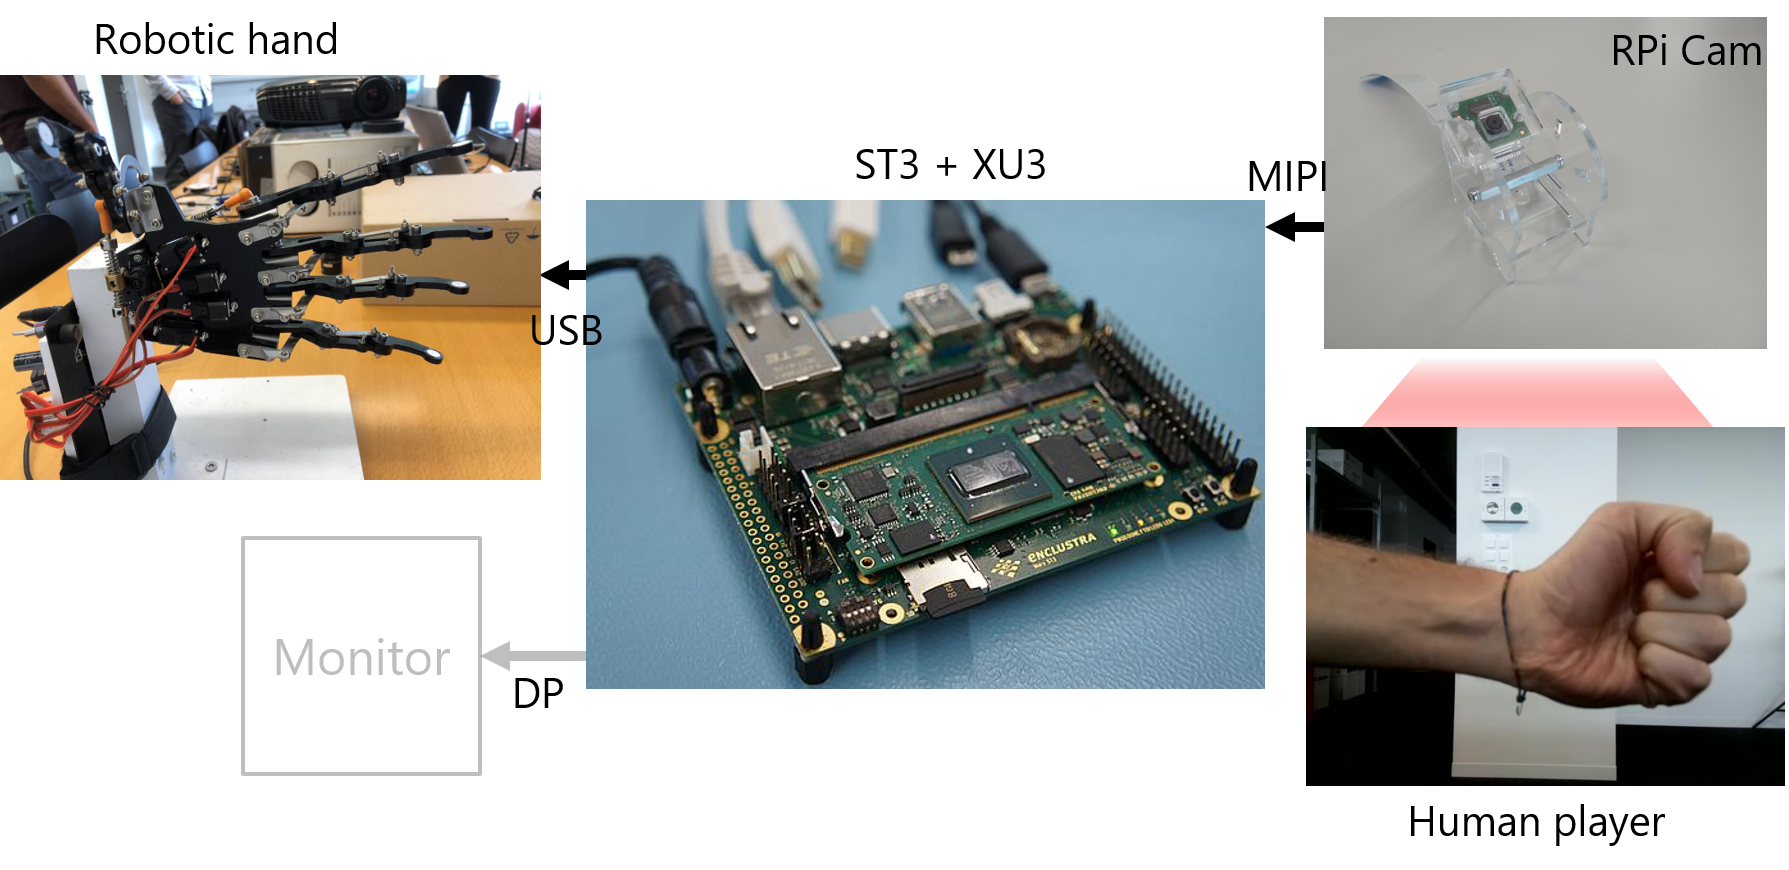
\includegraphics[width=\textwidth]{bilder/demonstrator.png}
		\caption{Rock-paper-scissors demonstrator setup}
		\label{fig:demonstrator}
	\end{figure}
\end{itemize}





\sloppy % avoid long urls in the border
\printbibliography


\appendix


% Appendix 
% Appendix 

\chapter{Tagesabläufe}











\end{document}